%% BioMed_Central_Tex_Template_v1.06
%%                                      %
%  bmc_article.tex            ver: 1.06 %
%                                       %

%%IMPORTANT: do not delete the first line of this template
%%It must be present to enable the BMC Submission system to
%%recognise this template!!

%%% loading packages, author definitions

%\documentclass[twocolumn]{bmcart}% uncomment this for two column layout and comment line below
\documentclass{bmcart}

\usepackage{mathptmx}       % selects Times Roman as basic font
\usepackage{helvet}         % selects Helvetica as sans-serif font
\usepackage{courier}        % selects Courier as typewriter font
\usepackage{type1cm}        % activate if the above 3 fonts are not available on your system
\usepackage{makeidx}         % allows index generation
\usepackage{graphicx}        % standard LaTeX graphics tool when including figure files
\usepackage{multicol}        % used for the two-column index
\usepackage[bottom]{footmisc} % places footnotes at page bottom
\usepackage{subfig}
\usepackage{amsfonts}
\usepackage[cmex10]{amsmath}
\usepackage{float}
\usepackage[utf8]{inputenc}

\usepackage{bm} 
\usepackage{amsmath}
\usepackage{amssymb}

\usepackage{caption}

%%%%%%%%%%%%%%%%%%%%%%%%%%%%%%%%%%%%%%%%%%%%%%%%%
%%                                             %%
%%  If you wish to display your graphics for   %%
%%  your own use using includegraphic or       %%
%%  includegraphics, then comment out the      %%
%%  following two lines of code.               %%
%%  NB: These line *must* be included when     %%
%%  submitting to BMC.                         %%
%%  All figure files must be submitted as      %%
%%  separate graphics through the BMC          %%
%%  submission process, not included in the    %%
%%  submitted article.                         %%
%%                                             %%
%%%%%%%%%%%%%%%%%%%%%%%%%%%%%%%%%%%%%%%%%%%%%%%%%

%\def\includegraphic{}
%\def\includegraphics{}

%%% Put your definitions there:
\startlocaldefs
\endlocaldefs

%%% Begin ...
\begin{document}

%%% Start of article front matter
\begin{frontmatter}

\begin{fmbox}
\dochead{Research}

% Document information

\title{Estimation of flow trajectories in a multi-lines network}

\author[
  addressref={aff1},                   
  corref={aff1},                       
  email={gguex@unil.ch}
]{\inits{G.G.}\fnm{Guillaume} \snm{Guex}}
\author[
  addressref={aff2},
  email={rloup@unil.ch}
]{\inits{R.L.}\fnm{Romain} \snm{Loup}}
\author[
addressref={aff1, aff2},
email={fbavaud@unil.ch}
]{\inits{F.B.}\fnm{François} \snm{Bavaud}}

\address[id=aff1]{%                           
  \orgdiv{Departement of Language and Information Sciences},             
  \orgname{University of Lausanne},          
  \city{Lausanne},                              
  \cny{Switzerland}                                   
}
\address[id=aff2]{%
  \orgdiv{Institute of Geography and Sustainability},
  \orgname{University of Lausanne},          
  \city{Lausanne},                       
  \cny{Switzerland} 
}

\end{fmbox}

% The Abstract begins here                  

\begin{abstractbox}

\begin{abstract} % abstract
Blabla
\end{abstract}

% Keywords begin here  

\begin{keyword}
\kwd{sample}
\kwd{article}
\kwd{author}
\end{keyword}

% MSC classifications codes, if any
%\begin{keyword}[class=AMS]
%\kwd[Primary ]{}
%\kwd{}
%\kwd[; secondary ]{}
%\end{keyword}

\end{abstractbox}

\end{frontmatter}

% Main Body

%% --------------------------------- INTRODUCTION

 

\section{Introduction}

\subsection{Context}

\subsection{Statement of the problem}

\subsection{Related Works}




%% --------------------------------- NOTATIONS AND FORMALISM

\section{Notations and formalism}
\subsection{Lines, stops  and junctions}
\label{Lines and junctions}
Consider a transportation network made of bus lines numbered $\ell=1,\ldots, q$, of respective lengths (number of stops) $l_\ell$.  Opposite lines, that is parallel lines running in the back and forth directions are considered as distinct. 

The $l=\sum_{\ell=1}^ql_\ell$ bus stops constitute the nodes of the transportation network. Each stop $i=1,\ldots,l$ belongs to {\em  a single bus line}, and defines a unique next or forward stop $F(i)$ (unless $i$ is the line terminus) and a unique backward stop $B(i)$ (unless $i$ is the line start), both on the same line.  

Let $S_i$ denote the set of stops which can be reached from stop $i$ within walking distance, excluding $i$ itself. A stop $i$ is referred to as an {\em isolated stop} if $S_i=\emptyset$, and to as a {\em junction} otherwise. 


\subsection{Line edges, transfer edges and trips}
\label{Line edges, transfer edges and trips}
Two sorts of oriented edges are involved in the transportation network: 
\begin{enumerate}
  \item[$\bullet$] intra-line edges $(i,j)=(i,F(i))$ belonging to a single line  $\ell(i)=\ell(j)$
  \item[$\bullet$] inter-line or transfer edges $(i,j)$ connecting different lines $\ell(i)\neq \ell(j)$, involving walks from junction $i$ to $j\in S_i$.
  \end{enumerate}
A $st$-trip, noted $[s,t]$, consists of entering into the network at stop $s$, and leaving the network at $t$, by following the shortest-path (i.e. achieving the minimum distance,  minimum time, or  minimum cost), supposed unique, leading to $s$ from $t$. 

The succession of edges $(ij)$ belonging to the $st$-trip, noted $(ij)\in [s,t]$, is unique. Define the edge-trip incidence matrix as
\begin{equation}
\label{edgetrip}
\chi_{ij}^{st} = \begin{cases}
  1    & \text{if $(ij)\in [s,t]$}, \\
  0    & \text{otherwise}.
\end{cases}
\end{equation}
A $st$-trip always starts with the edge $(s,F(s))$, and finishes with $(B(t),t)$. Transfers can occur in-between, but never at the beginning nor at the end of the trip. 

\vspace*{0.1cm}

\subsection{Transportation flows}
\label{Transportation flows}
Let  $x_{ij}$ count the number of travelers using edge $(ij)$ in a given period, such as a given hour, day, week or  year.  The edge flow $x_{ij}$ is denoted by $y_{ij}$ for an intra-line edge $(i,j)$, and 
by $z_{ij}$ for a transfer edge $(i,j)$. By construction, $x_{ij}=y_{ij}+z_{ij}$, where $y_{ij}\,  z_{ij}=0$. 

\vspace*{0.1cm}


Let $a_i$, respectively $b_i$, the number of passengers embarking, respectively disembarking at stop $i$. By construction, 
\begin{equation}
\label{bilan1ligne}
\begin{cases}
 y_{i,F(i)}=a_i \text{\,  and } b_i=0   & \text{if $i$ is a line start}, \\
y_{B(i),i}=b_i \text{\,  and } a_i=0   & \text{if $i$ is a line terminus}, \\
 y_{i,F(i)}=y_{B(i),i}+a_i-b_i     & \text{otherwise}.
\end{cases}
\end{equation}
Also, $\mathbf{a}$ and $\mathbf{b}$ must be consistent, in the sense that $A_i\ge B_i$, where $A_i$ (respectively $B_i$) is the cumulated number of embarked 
(resp. disembarked) passengers on the line under consideration, recursively defined as $A_{F(i)}=A_i+a_i$ (resp. $B_{F(i)}=B_i+b_i$). Moreover,  $A_i=B_i$ at a terminal line stop $i$. This common value yields  the total number of passengers transported by the line. 



\vspace*{0.1cm}

Let the transportation flow $n_{st}$ denote the number of passengers following an $st$-trip, that is entering the network at $s$ and leaving the network at $t$ by using the shortest path. One gets from (\ref{edgetrip}) 
\begin{equation}
\label{equationGG}
x_{ij}=\sum_{st}\chi_{ij}^{st}\:  n_{st}
\end{equation}
Among the passengers embarking in $i$, some transfer from another line, and some others enter into the network: 
\begin{equation}
\label{entrer}
a_i=z_{\bullet i}+n_{i\bullet}
\end{equation}
where  ``$\bullet$" denotes the summation over the replaced index, as in $n_{i\bullet}=\sum_{j=1}^l n_{ij}$. Similarly, among the passengers disembarking in $i$, some transfer to another line, and some others leave the network: 
\begin{equation}
\label{sortir}
b_i=z_{i\bullet}+n_{\bullet i}
\end{equation}
By construction
\begin{displaymath}
a_{\bullet}=b_{\bullet}=z_{\bullet\bullet}+n_{\bullet\bullet}
\end{displaymath}
where $n_{\bullet\bullet}$ counts the number of passengers, and $z_{\bullet\bullet}$ counts the number of transfers. $z_{\bullet\bullet}/n_{\bullet\bullet}$  is the average number of transfers per passenger. 

\vspace*{0.1cm}



As explained in section \ref{Lines and junctions}, transfers can only occur at junctions, that is $z_{ij}>0$ implies $j\in S_i$. In particular,  $z_{ii}=0$ : no traveller is supposed to disembark and re-embark later at the same stop. 


 
\subsection{Statement of the problem and solution method}
Automatic passenger counters measure the number of passengers entering and leaving buses at each stop [Boyle, 1998], that is $\mathbf{a}$ and $\mathbf{b}$, which provide the basic raw data of the present study, kindly provided by the Lausanne Transportation Agency (tl), after some preliminary, undocumented corrections (i.e. the components of $\mathbf{a}$ and $\mathbf{b}$ can be non-integer). It may also happen that raw data do not obey the necessary consistency condition  $a_\bullet=b_\bullet$, in which case we did rescale the embarking and disembarking counts as 
\begin{displaymath}
\hat{a}_i=\varepsilon a_i \qquad\qquad \hat{b}_i=\frac{1}{\varepsilon} b_i \qquad\qquad\mbox{with}\quad \varepsilon=\sqrt{\frac{b_\bullet}{a_\bullet}}
\end{displaymath}
ensuring $\hat{a}_\bullet=\hat{b}_\bullet$, unless $\varepsilon> 2$ or $\varepsilon<\frac{1}{2}$ ***@R, @G : c'est à peu près cela??*** , in which case the corresponding line (which always turned out to be a temporary line with small  counts) was simply disregarded and removed from the network. 


Also, the geometry of the network permits to derive the edge-trip incidence matrix $\bm{\chi}$ defined in (\ref{edgetrip}). 


Intra-line edge flows $\mathbf{Y}=(y_{ij})$ can be determined by (\ref{bilan1ligne}), but transfer edge flows $\mathbf{Z}=(z_{ij})$ are, here and typically, unknown. The objective is to estimate the $l\times l$ transportation flow $\mathbf{N}=(n_{st})$. Many consistent solutions coexist in general, even for a single line with no transferts (section \ref{Single line}). This issue of incompletely observed data can be tackled by the maximum entropy formalism \cite{jaynes1957information}, and has been often  in transportation modelling \cite{wilson1967statistical}  \cite{erlander1990gravity}. Its contemporary justification corresponds to the ``expectation step" of the EM algorithm \cite{dempster1977maximum}  \cite{bavaud2009information}. 




Let $f_{st}=n_{st}/n_{\bullet\bullet}$ be the proportion of $st$-trips (empirical distribution) and let $g_{st}$ be some prior guess on its shape (theoretical distribution). 
Assuming some reasonable initial prior $g_{st}$, 
\begin{itemize}
\item[(1)] we shall first suppose that the empirical margins $\alpha_s=f_{s\bullet}$ and $\beta_t=f_{\bullet t}$ are known.  
Then $f_{st}$ can be determined as the maximum entropy solution (section \ref{maxenso}), i.e. as the distribution closest to $g_{st}$ in the Kullback-Leibler divergence sense under the margin constraints
\item[(2)] then (section \ref{marginup}), the margins will be updated to $\tilde{\alpha}_s$ and $\tilde{\beta}_t$   by requiring a minimum proportion $\theta\in (0,1)$ of passengers entering/leaving the network at each stop, as well as avoiding transfer overflow exceeding the embarking and disembarking counts at each stop
 \item[(3)] finally (section \ref{priorup}), the prior will be updated to $\tilde{g}_{st}$ by shrinking, if necessary, the priors $g_{st}$ associated to overflows. 
\end{itemize}
With the new prior distribution $\widetilde{g}_{st}$ and the new margin distributions $\widetilde{\alpha}_s$, $\widetilde{\beta}_t$, we can iterate the 
 the above steps, until convergence. The only free parameter is $\theta$, which will be discussed in section *** . *** This solution method is reminiscent, but quite distinct of the ME algorithm ...***




\subsubsection{Maximum entropy estimate of $st$-trips}
\label{maxenso}
As announced,  the proportion of $st$-trips $f_{st}=n_{st}/n_{\bullet\bullet}$ (empirical distribution) will be estimated from some prior guess $g_{st}$ (theoretical distribution) and 
margin constraints $\alpha_s$ and $\beta_t$ for $f_{st}$ by maximum entropy, i.e. by 
solving the problem 
\begin{align}
	\label{constr_MaxEnt}
	\min_{\mathbf{f}\in\mathcal{F}} &\; \sum_{st}f_{st}\log \frac{f_{st}}{g_{st}}, \notag \\
	s.t. &\; \sum_t f_{st} = \alpha_s, \notag \\
	&\; \sum_s f_{st} = \beta_t.
\end{align}
The Lagragian is
\begin{equation}
	L = \sum_{st}f_{st}\log \frac{f_{st}}{g_{st}} - \sum_s \lambda_s (\alpha_s - \sum_t f_{st}) - \sum_t \mu_t (\beta_t - \sum_s f_{st}), \notag
\end{equation}
which gives, after deriving and setting to zero,
\begin{equation}
	\label{Sol}
	f_{st} = \phi_s \psi_t g_{st} \qquad \text{with } \phi_s := \exp(- 1 - \lambda_s) \text{, } \psi_t := \exp(- \mu_t).
\end{equation}
Using constraints in (\ref{constr_MaxEnt}), we find
\begin{equation}
	\label{Sol_LagMult}
	\phi_s = \frac{\alpha_s}{\sum_t \psi_t g_{st}}, \qquad \psi_t = \frac{\beta_t}{\sum_s \phi_s g_{st}}, 
\end{equation}
which yields the following \emph{iterative fitting algorithm}: starting with some $\psi^{(0)}_t > 0$, one performs the iteration
\begin{equation}
	\label{Iterative fitting}
	\phi^{(\iota)}_s = \frac{\alpha_s}{\sum_t \psi^{(\iota)}_t g_{st}}, \qquad \psi^{(\iota + 1)}_t = \frac{\beta_t}{\sum_s \phi^{(\iota)}_s g_{st}}, 
\end{equation}
until convergence to $\phi_s$ and $\psi_t$ obeying (\ref{Sol_LagMult}). 

In view of (\ref{entrer}) and (\ref{sortir}), the postulated margins must satisfy, for each isolated stop $i$
\begin{equation}
\label{ }
\alpha_i=\frac{a_i}{n_{\bullet \bullet}}\qquad\qquad \beta_i=\frac{b_i}{n_{\bullet \bullet}}
\end{equation}
permitting to determine the total flow as $n_{\bullet \bullet}=\frac{a_i}{\alpha_i}$, or  $n_{\bullet \bullet}=\frac{b_i}{\beta_i}$ for any isolated stop $i$, and thus 
the $st$-flow itself as 
\begin{equation}
	\label{flow_from_distrib}
	n_{st} = n_{\bullet \bullet} f_{st}= n_{\bullet \bullet}\phi_s \psi_t g_{st} 
\end{equation}
whose plugging into (\ref{equationGG}) yields the intra-line edge flows $\mathbf{Y}=(y_{ij})$ and the transfer edge flows $\mathbf{Z}=(z_{ij})$.


\subsubsection{Initialization of the prior and the margins}
The geometry of the network permits to rule out forbidden $st$-paths, i.e. obeying  $\chi^{st}_{\bullet\bullet}=0$. Such forbidden $st$-paths consist of *** @G? donner une liste exhaustive de critères d'exclusion ici ? ***  The initial prior was chosen as the uniform distribution on the remaining $c<l^2$ admissible $st$-paths, *** @G: que vaut $l$? que vaut $c$? ***,  that is as
\begin{equation*}
g_{ij} = \begin{cases}
  \frac{1}{c}    & \text{if $\chi^{st}_{\bullet\bullet}>0$}, \\
  0    & \text{otherwise}.
\end{cases}
\end{equation*}
The initial margins were chosen as  those of the flow without transfer, namely $\alpha_i=\frac{a_i}{a_{\bullet}}$ and $\beta_i=\frac{b_i}{b_\bullet}$ for all stops. 



\subsubsection{Updating  the margin distributions}
\label{marginup}
Let us define the hyperparameter $ \theta\in [0, 1)$ as the \emph{minimum proportion of passengers (among $a_i$ and $b_i$) entering/leaving the network at each stop}, that is $n_{s\bullet}\ge \theta a_s$ and $n_{\bullet t}\ge \theta b_t$. Note that we could set a different hyperparameter for each node, and differing for embarkments and disembarkments, but without addition information, we will restrain to this simpler case. Identities (\ref{entrer}) and  (\ref{sortir}) then imply the inequalities
\begin{displaymath}
z_{\bullet s} \le (1 - \theta) a_s\qquad\qquad \qquad z_{t \bullet} \le  (1 - \theta) b_t
\end{displaymath}
the violation of which constitutes transfer overflow. Hence requiring a minimal transfer yet avoiding overflow can be granted with the following updating of margins
\begin{equation}
\label{alpha_beta_update}
\widetilde{\alpha}_s = \frac{\min(\theta a_s, a_s - z_{\bullet s})}{\sum_{s'} \min(\theta a_{s'}, a_{s'} - z_{\bullet {s'}})}   \qquad \qquad \qquad
	\widetilde{\beta}_t = \frac{\min(\theta b_t, b_t - z_{t \bullet})}{\sum_{t'} \min(\theta b_{t'}, b_{t'} - z_{{t'} \bullet})}  \enspace. 
\end{equation}
 

\subsubsection{Updating the prior distribution}
\label{priorup}
Overflow occurs in transfer edge $(i, j)$ if  $z_{i \bullet} > (1 - \theta)b_i$ or $z_{\bullet j} > (1 - \theta)a_j$. To avoid it, components $g_{st}$ of the prior distribution 
will be shrinked by a suitable ratio whenever edge flows $(i,j)\in [s,t]$ exhibit overflow. 


 For any edge $(i, j)$, let us compute the \emph{flow ratio} $r_{ij}$ as
\begin{equation}
	\label{flow_ratio}
	r_{ij} = \max \left(1, \frac{z_{i \bullet}}{(1 - \theta)b_i}, \frac{z_{\bullet j}}{(1 - \theta)a_j} \right)\: \ge\: 1\enspace,
\end{equation}
where $r_{ij} > 1$ denotes an overflow through edge $(i, j)$. For a given origin-destination $[s,t]$, define the \emph{orgin-destination flow ratio} $\bar{r}_{st}$ 
as the largest $r_{ij}$ among edge flows $(i,j)\in [s,t]$, that is as 
\begin{equation}
	\label{st_flow_ratio}
	\bar{r}_{st} = \max_{ij} \chi_{ij}^{st} r_{ij}\: \ge\: 1\enspace.
\end{equation}
By construction, $\bar{r}_{st} > 1$ denotes an overflow on some transfer edge between $s$ and $t$. To adjust the flow, we shall divide the previous flow by this ratio
\begin{equation}
	\label{update_flow}
	\widetilde{n}_{st} =\frac{n_{st}}{\bar{r}_{st}}
\end{equation}
and define the new prior distribution  as
\begin{equation}
	\label{update_distrib}
	\widetilde{g}_{st} = \frac{\left( \frac{\widetilde{n}_{st}}{\phi_s \psi_t} \right)}{\sum_{s',t'} \left( \frac{\widetilde{n}_{s',t'}}{\phi_{s'} \psi_{t'}} \right)}\enspace. 
\end{equation}
where $\phi_s$ and $\psi_t$ are the values (\ref{Sol_LagMult}) obtained in the previous maximum entropy step. 





\subsection{The case of a single line}
\label{Single line}
A ``network" made of a single line contains no transfers, and flow estimates can be obtained at once by the maximum entropy step only.


Let  $i=1,\ldots, l$ enumerate the bus stops in increasing order,  i.e. $F(i)=i+1$. The initial prior is simply $g_{st}=\frac{I(s<t)}{(l-1)(l-2)}$ (where $I(.)$ denotes the 0/1  indicator function), capturing solely the unidirectional nature of trips. The margins of the empirical distribution $f_{st}$, as well as the total flow, are here known : 
\begin{displaymath}
\alpha_s=\frac{a_s}{a_\bullet}\qquad\qquad\qquad \beta_t=\frac{b_t}{b_\bullet}\qquad\qquad\qquad n_{\bullet\bullet}=a_{\bullet}=b_\bullet
\end{displaymath}
and (\ref{Sol}) yields, after reparameterization, maximum entropy flows of the form
\begin{equation}
\label{nosignle}
n_{st}=I(s<t)\, c_s\, d_t \qquad\qquad\mbox{where}\quad \sum_{s}c_s\, \sum_{t>s}d_t=n_{\bullet\bullet}
\end{equation}
where (setting $D_s:=\sum_{t>s}d_t$ and $C_t:=\sum_{s<t}c_s$) the constraints (\ref{Sol_LagMult}) equivalently express as 
\begin{equation}
\label{dis embarking constraints}
c_s=\frac{a_s}{\sum_{t>s}d_t}=\frac{a_s}{D_s}
\qquad\qquad\qquad
d_t=\frac{b_t}{\sum_{s<t}c_s}=\frac{b_t}{C_t}
\end{equation}
to be solved by iterative fitting. 

Interestingly enough, the form (\ref{nosignle}) for the flows is reminiscent of the {\em gravity flows} of quantitative Geography \cite{wilson1967statistical}  \cite{erlander1990gravity} \cite{bavaud2002quasi}, where 
$c_s$ is the {\em push factor}, $d_t$ is the {\em pull factor}, and $I(s<t)$ the {\em distance deterrence function}. Yet, instead of  
being symmetric in $s,t$ and decreasing with the distance $|s-t|$, the distance deterrence function is here asymmetric due to the line orientation, but otherwise constant. 

This constancy entails the following Markovian behaviour for flows: let $m_{st}$ be the number of travelers embarking at stop $s$ and still inside the bus at stop $t>s$, and let $\rho_{st}$ the probability that travelers embarking at $s$ will disembark at $t$. By (\ref{nosignle}), 
\begin{displaymath}
m_{st}=\sum_{u\ge t}n_{su}=c_s \sum_{u\ge t} I(s<u)\, d_u =c_s (d_t+D_t) 
\end{displaymath}
The empirical estimate of $\rho_{st}$ is given by the proportion, among the travelers embarking at $s$ and 
 still present at $t>s$,  of travelers disembarking at $t$, that is 
\begin{displaymath}
\rho_{st}=\frac{n_{st}}{m_{st}}=\frac{c_s\,  d_t}{c_s\,  (d_t+D_t)}=\frac{d_t}{d_t+D_t}=\frac{b_t}{C_t\, (d_t+D_t)}\le 1
\end{displaymath}
which depends on $t$ only: it  finally  turns out that the disembarkment probability $\rho_t=\frac{d_t}{d_t+D_t}$ at $t$ is {\em independent} of the embarkment stop $s$. Said otherwise, a traveler embarking at any stop $s$ (and thus necessarily in the bus at $F(s)=s+1$) experiences the {\em same disembarkment probability} at each  stop $t$. 


This Markov property, enjoyed by maximum-entropic flows, contrasts other possible solutions, such as  the ``first in, first out" (FIFO) flows (homogenizing the 
traveled distances among users) or the ``last in, first out" (LIFO) flows (tending to generate maximally  contrasted traveled distances).

\


***  @G, ici davantage de développements sur l'approche Markovienne, ainsi que le joli schéma ?  ***


\

*** @G, @R, ici la (les) figure de l'exemple  ``starting from Maladière, Riant-Cour, Dapples"... ? ***

 
%% --------------------------------- CASE STUDIES

\section{Case Studies}


\subsection{Toy Examples}

\subsection{Real Data}

%% --------------------------------- CONCLUSION

\section{Conclusion}

  
\newpage

\section*{Previous submission to complex networks 2022}

%
\section*{Statement of the problem}
%

Automatic passenger counters measure the number of passengers entering and leaving buses at each stop \cite{boyle_passenger_1998}. Given this information, can we estimate the complete trajectories of passengers within the entire multi-line network? This communication attempts to propose an estimation of all passenger trajectories in the multi-line network with an algorithm based on iterative proportional fitting (IPF) \cite{bishop_discrete_2007}.

The exploited dataset is provided by the Lausanne Transportation Agency (tl) in Switzerland. The dataset includes 42 lines of buses (or subways) and more than 1361 stops, including 497 clusters of stops (Fig. \ref{fig:map-lausanne}),  carrying around 115 million passengers in 2019. Each stop refers to a single directed line, and return lines are considered as distinct.  In addition to  \emph{line edges},  it is possible to construct pedestrian \emph{transfer edges} (Fig. \ref{fig:network-lausanne}) to make the graph unilaterally connected by considering, e.g., clusters of stops connected.

\noindent \begin{minipage}[c]{0.5\textwidth}
   \begin{figure}[H]
      \centering
      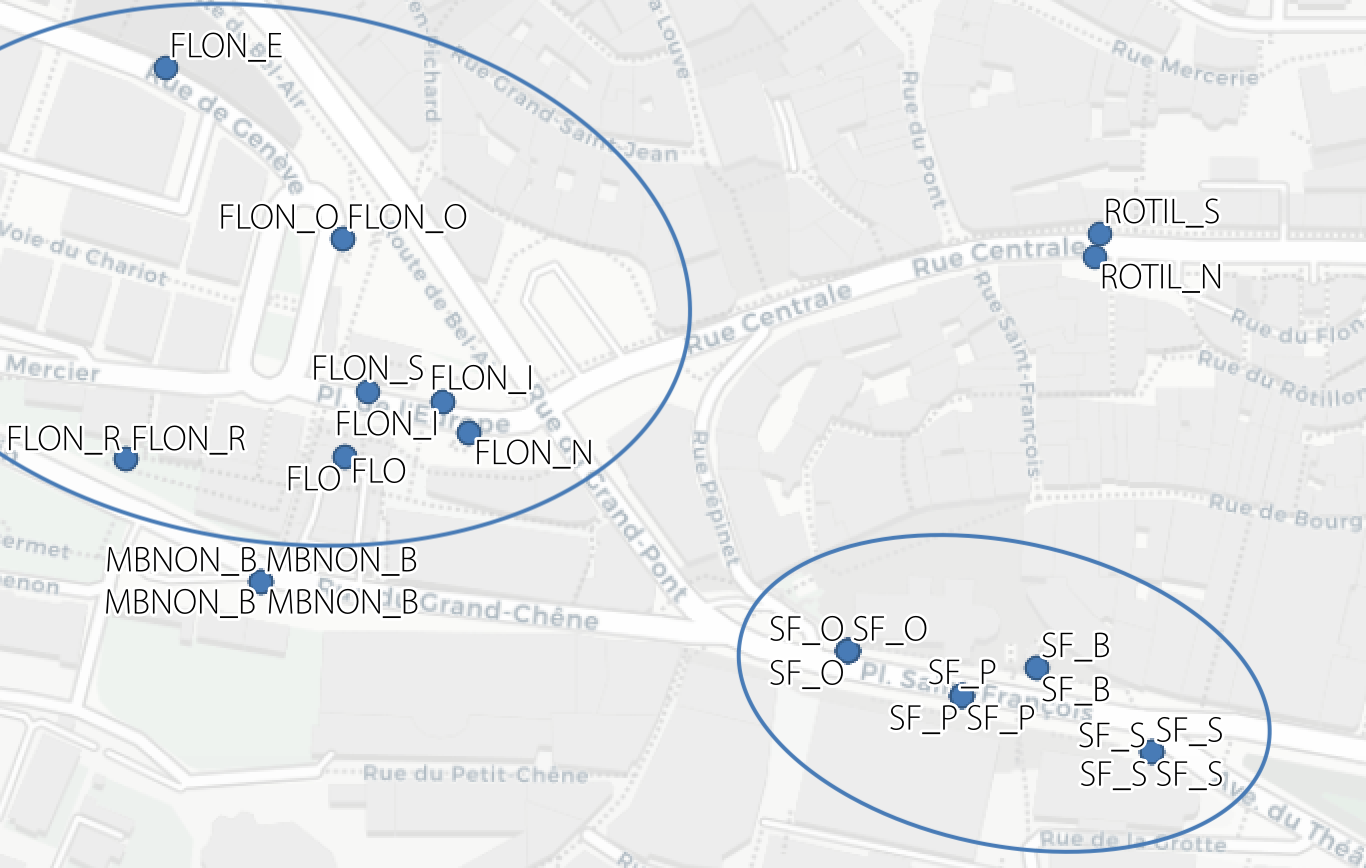
\includegraphics[width=6cm]{img/stop_area_c.png}
      \caption{Cluster of stops} 
      \label{fig:map-lausanne}
   \end{figure}
\end{minipage}%
\begin{minipage}[c]{0.5\textwidth}
   \begin{figure}[H]
      \centering
      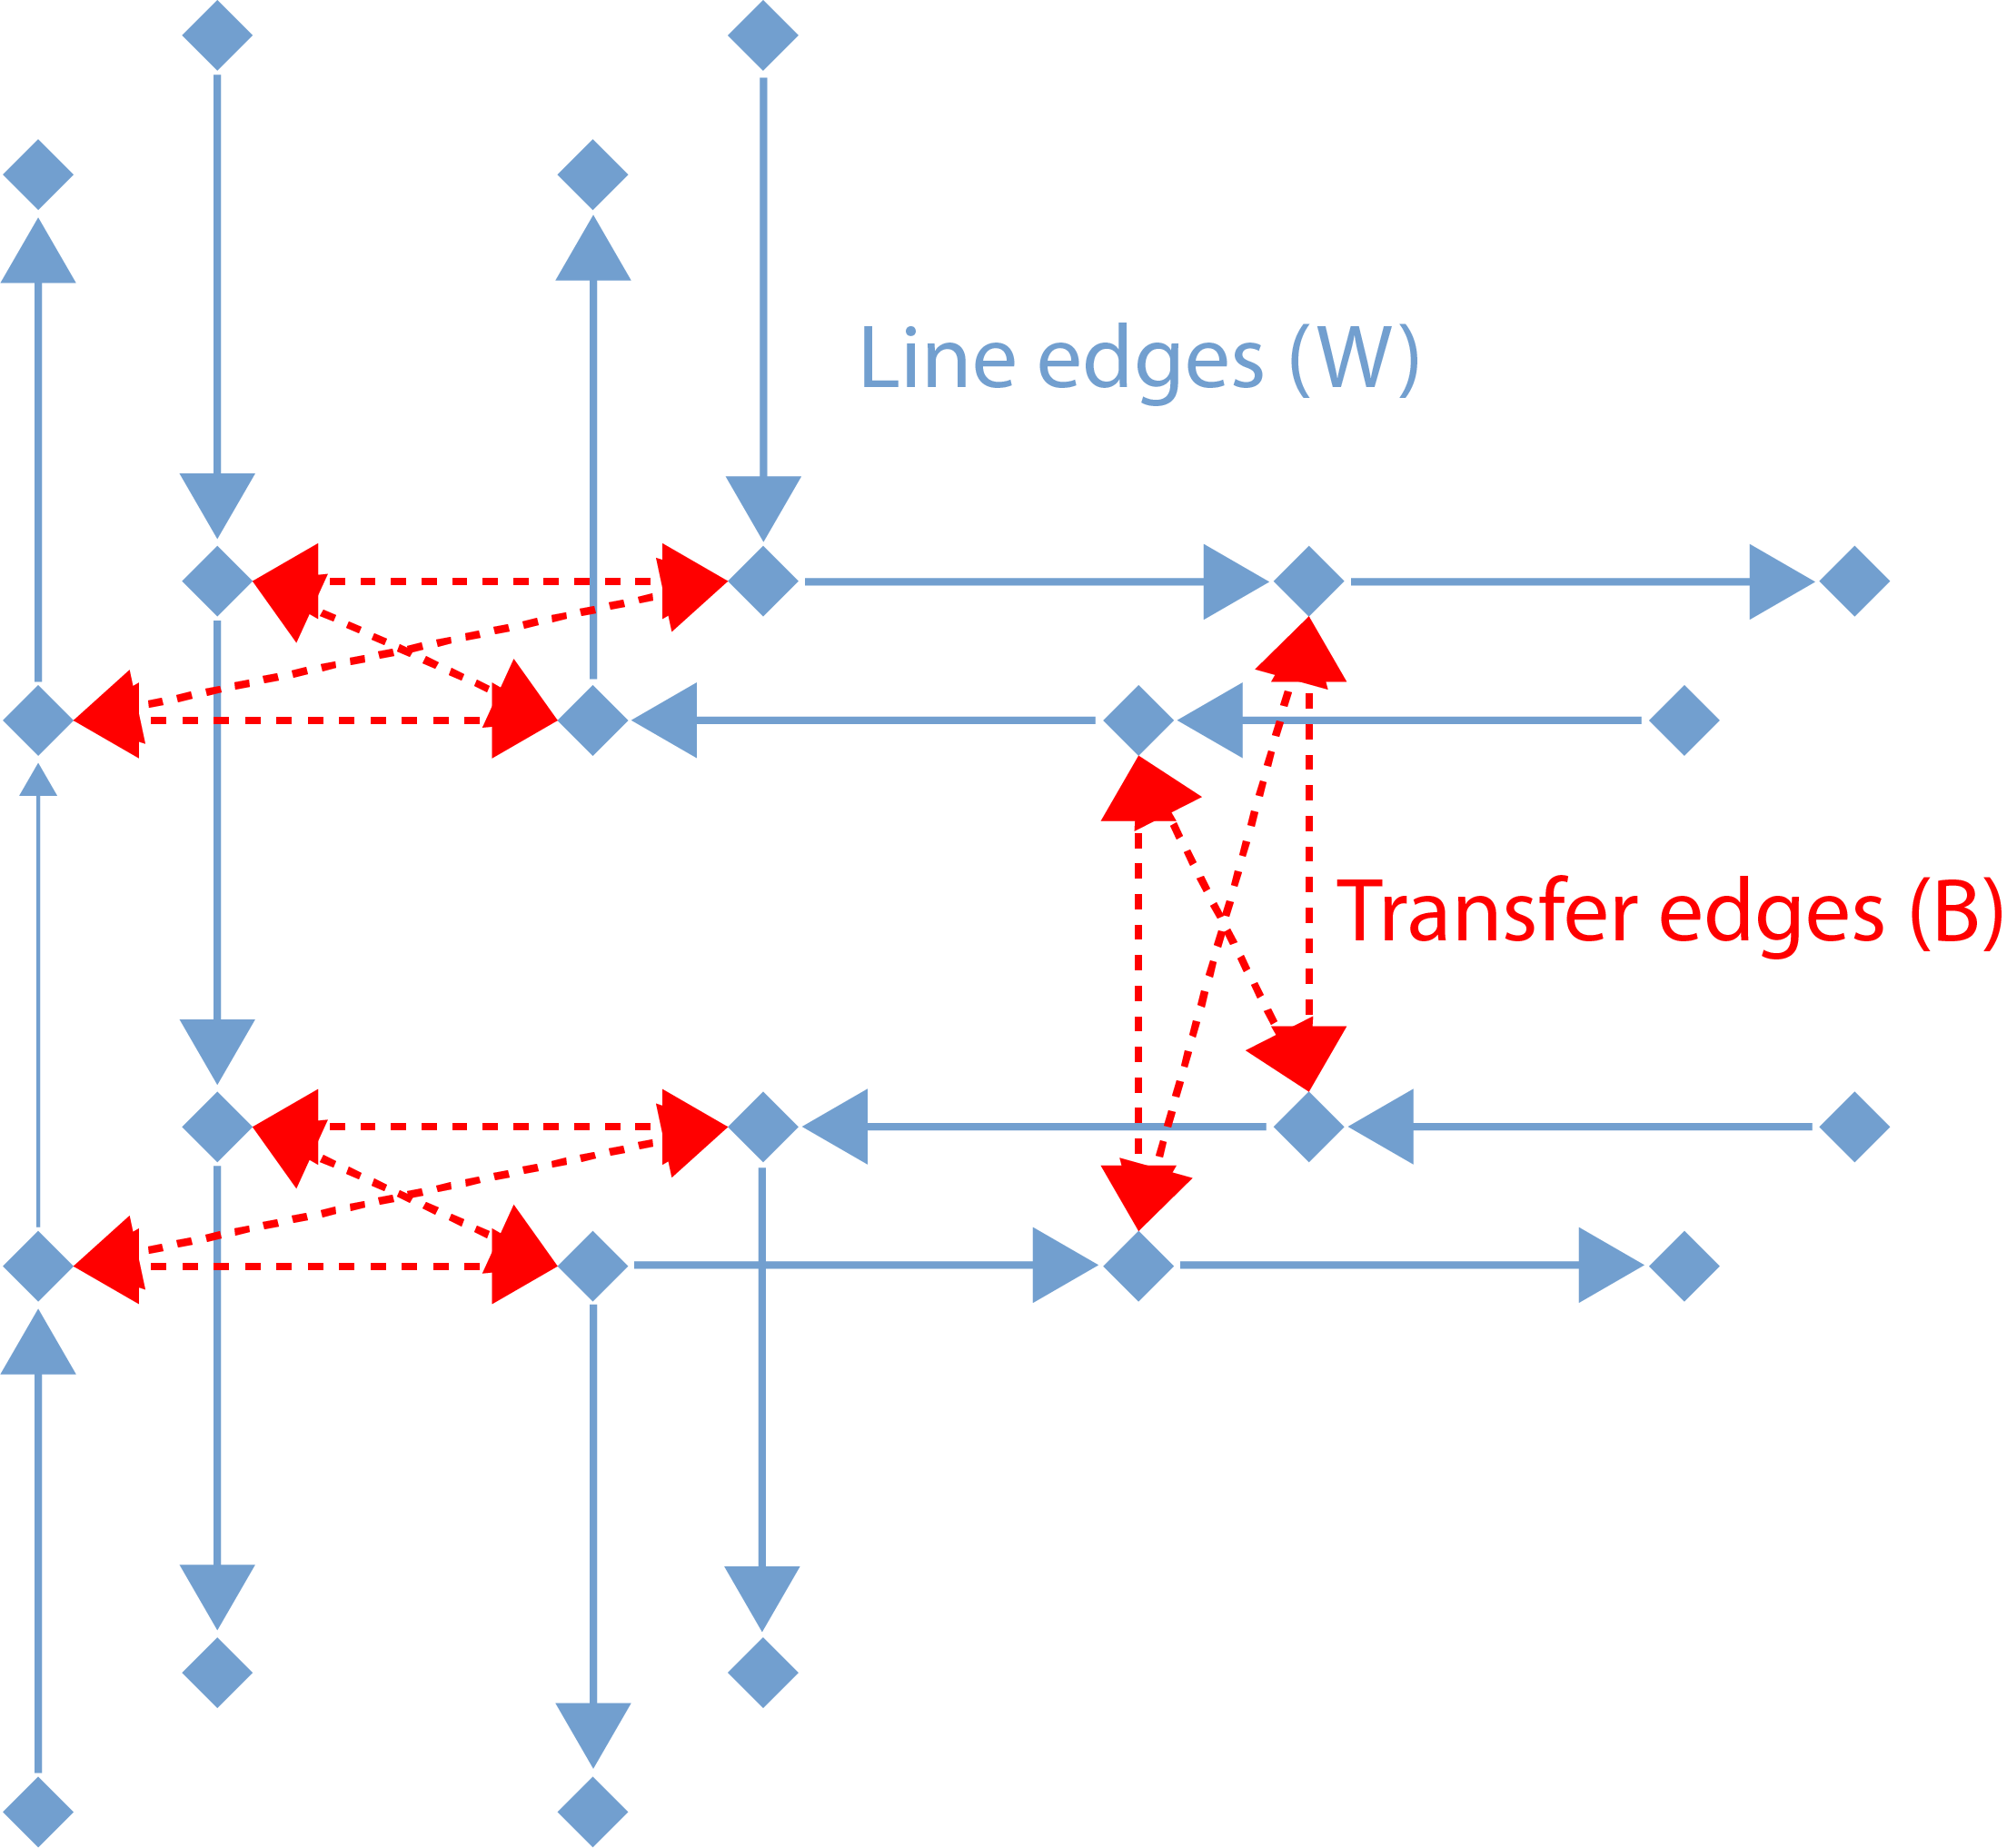
\includegraphics[width=4cm]{img/edge_type3.png}
      \caption{The multi-line network structure} 
      \label{fig:network-lausanne}
   \end{figure}
\end{minipage}


$\mbox{}$

Knowing only the network structure and the number of passengers embarking and disembarking at each stop, how can we infer the most probable passenger trajectories in the network? Before examining the general multi-line network problem,  we address the estimation of trajectories on a single line.

%
\section{Single line}
%

Consider a one-directional line with $n$ stops indexed regarding the order found in the line.  Let $\mathbf{a}_\text{in} = (a_{s}^\text{in})$ and $\mathbf{a}_\text{out} = (a_{t}^\text{out})$ be two vectors representing, respectively, the passengers entering and leaving the line at each stop. The goal is to estimate the $(n \times n)$ origin-destination matrix $\mathbf{N} = (n_{st})$, where $n_{st}$ represents the number of passengers entering the line at $s$ and leaving at $t$, subject to constraints $n_{s\bullet} = a^\text{in}_s$ and $n_{\bullet t} = a^\text{out}_t$.  Among many feasible solutions, arguably the most elegant one is the maximum entropy solution, which can be derived  from different means:  (i) passenger flows can be modelled using a Markovian assumption, which translates by assuming that every passenger has the same probability to continue the trip after having travelled at last one stop ; (ii) an iterative proportional fitting algorithm can be performed, starting with an initial origin-destination affinity matrix $\mathbf{S} = (s_{st})$, defined as the upper triangular $n\times n$ matrix filled with $1$, and then iterated to satisfy the margin constraints given by $\mathbf{a}_\text{in}$ and $\mathbf{a}_\text{out}$. Both approaches give the same solution, but only the latter remains pertinent in the multi-line problem.

%
\section{Multi-lines}
%

In the multi-line problem, a passenger can transfer from a line to another. The problem cannot be tackled with Markov chain modelling anymore, which generate unrealistic random trajectories. Instead, we will assume that passengers follow shortest paths. Starting from an origin-destination matrix $\mathbf{N} = (n_{st})$, where $s$ denotes the stop at which a passenger \emph{enters into the network} (and not simply enters a particular line), and $t$ denotes the stop where the passenger \emph{leaves definitively the network}, this shortest paths assumption allows us to compute the flow matrix on edges $\mathbf{X} = (x_{ij})$. The latter decomposes into the within-line flow and the transfer flow, i.e., $\mathbf{X}=\mathbf{X}_\text{W}+\mathbf{X}_\text{B}$. 
Moreover, in the multi-line problem, we also have to distinguish between:
\begin{itemize}
	\item[$\bullet$]  passengers who enter and leave bus lines at each stop, represented by vectors $\mathbf{a}_\text{in}$ and $\mathbf{a}_\text{out}$, which are \emph{measured},
	\item[$\bullet$] and passengers who enter and leave the network at each stop $i$, represented by the \emph{unknown} quantities $n_{\bullet i}$ and $n_{i \bullet}$.
\end{itemize}
By construction, 
\begin{align}
		a^\text{in}_i &=n_{i\bullet} + x^\text{B}_{i\bullet},  &
		a^\text{out}_i &= n_{\bullet i} + x^\text{B}_{\bullet i},
\end{align}

Using these two constraints, along with the shortest paths assumption and iterative proportional fitting, we propose the following iterative algorithm in order to find $\mathbf{N}$ from measured $\mathbf{a}_\text{in}$ and $\mathbf{a}_\text{out}$. \\

\noindent \fbox{\begin{minipage}{\textwidth}

\textbf{Initialisation:} $\mathbf{S}^{(0)}$ is filled with 1 excepted for aberrant origin-destination pairs (such as $t$ beeing a previous stop of the same line as $s$). The margins of $\mathbf{N}$ are fixed as $\mathbf{n}^{(0)}_{\mbox{\scriptsize in}} = \mathbf{a}_\text{in}$ and $\mathbf{n}^{(0)}_{\mbox{\scriptsize out}} = \mathbf{a}_\text{out}$.

\textbf{Step 1, Iterative proportional fitting:}
We use IPF to compute $\mathbf{N}^{(r)}$ starting from $\mathbf{S}^{(r)}$, such that margin constraints, defined by $\mathbf{n}^{(r)}_\text{in}$ and $\mathbf{n}^{(r)}_\text{out}$ are satisfied.

\textbf{Step 2, Shortest paths flow:}
Using shortest paths information, we compute $\mathbf{X}^{(r)}_\text{B}$ from $\mathbf{N}^{(r)}$.

\textbf{Step 3, Affinity and margin update:}
$\mathbf{S}^{(r+1)}$, $\mathbf{n}^{(r+1)}_\text{in}$ and $\mathbf{n}^{(r+1)}_\text{out}$ are updated in order to respect constraints defined by (1).
\end{minipage}}

Step 1, 2, and 3 are iterated until convergence, giving an admissible solution to the problem.
%
\section{A small example}
%

As an illustration, an estimated solution proposed by the algorithm on a restricted network made of four lines only is depicted on Fig. \ref{fig:example-map}. A total of $n_{\bullet \bullet} = 16,837,494$ passengers using this network is estimated by the algorithm. The red circle on the bottom left represents the start of the trip $s$ and the size of the circles at stops $t$ represents the estimated number of passengers terminating their trip at $t$. In this example, the majority of passengers exit the network on the same initial embarkment line. A small fraction of them takes another line. 

Table \ref{fig:example-edges} represents the estimated ten most frequented transfer edges. The code of the stop represents the number of the line, the direction and a condensed name of its stop cluster. The third column gives the number (in thousands) of passengers transferring through this edge.

\noindent \begin{minipage}[c]{0.6\textwidth}
   \begin{figure}[H]
      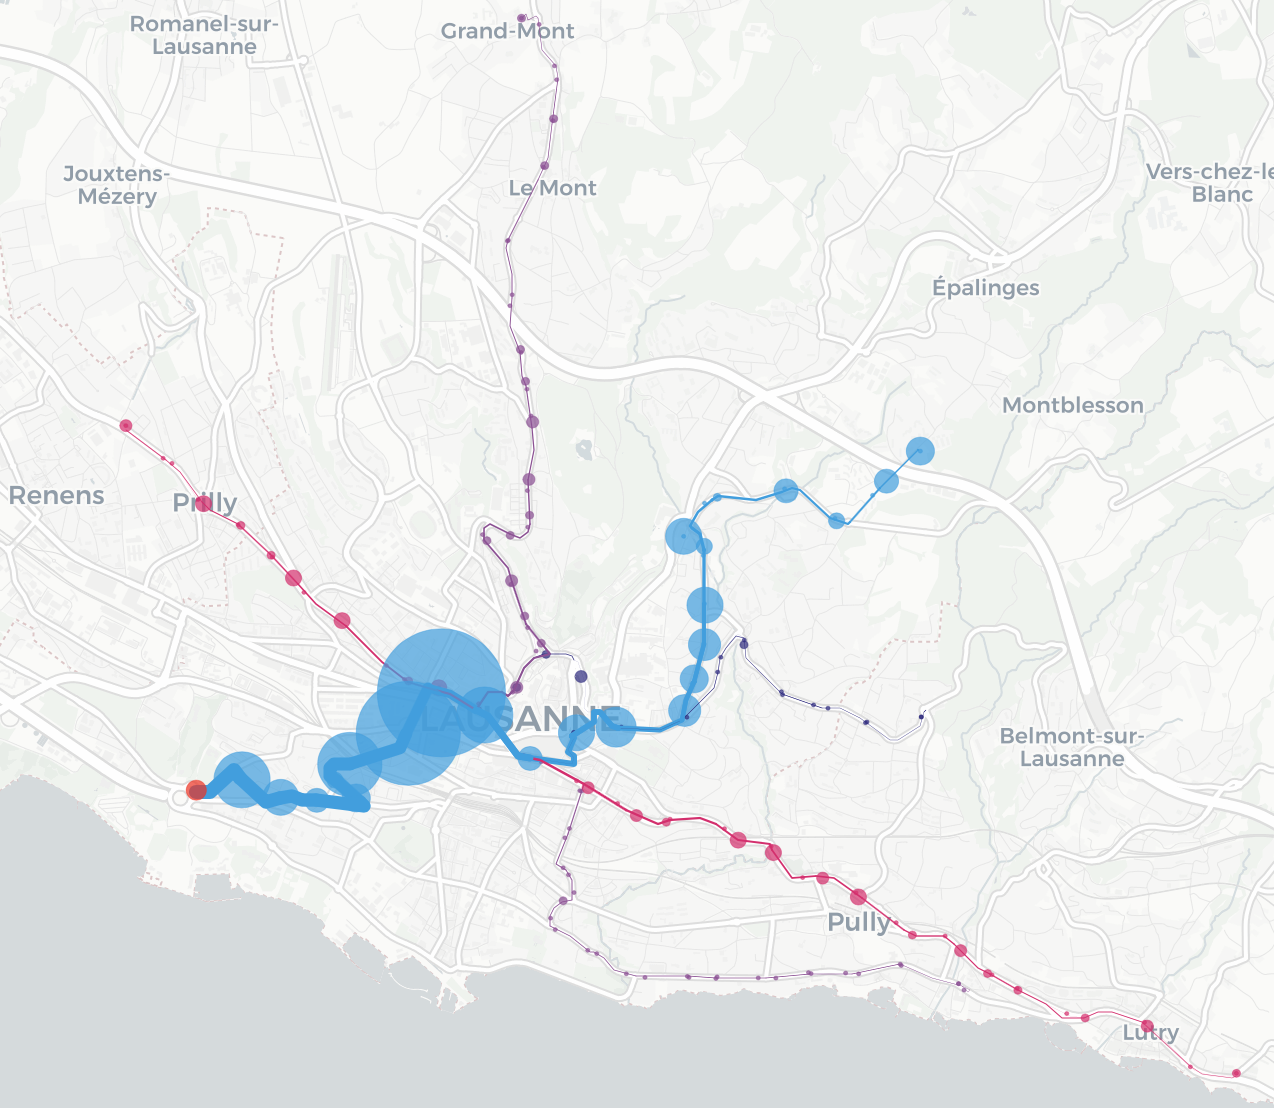
\includegraphics[width=7cm]{img/example_map.png}
      \caption{Example map} 
      \label{fig:example-map}
   \end{figure}
\end{minipage}%
\begin{minipage}[c]{0.43\textwidth}
      %\centering
      \begin{table}[H]
		\begin{tabular}{l|l|r}
		\multicolumn{1}{c|}{\textbf{From stop}} & \multicolumn{1}{c|}{\textbf{To stop}} & \multicolumn{1}{c}{\textbf{Count}} \\ \hline
		{\scriptsize S7\_A\_SF\_O}			& {\scriptsize S9\_A\_SF\_O}			& 192k		\\ \hline
		{\scriptsize S9\_R\_CH\_E}			& {\scriptsize S6\_A\_CH\_E}			& 187k		\\ \hline
		{\scriptsize S7\_A\_SF\_O}		& {\scriptsize S8\_R\_SF\_S}				& 135k			\\ \hline
		{\scriptsize S6\_R\_CH\_O}			& {\scriptsize S9\_A\_CH\_O}			& 135k			\\ \hline
		{\scriptsize S8\_A\_GTE\_N}		& {\scriptsize S9\_R\_GTE\_E}			& 103k		\\ \hline
		{\scriptsize S9\_R\_B-AIR\_C}		& {\scriptsize S8\_A\_B-AIR\_N}		& 99k			\\ \hline
		{\scriptsize S9\_A\_SF\_O}			& {\scriptsize S7\_A\_SF\_O}			& 88k			\\ \hline
		{\scriptsize S8\_R\_B-AIR\_D}		& {\scriptsize S6\_A\_B-AIR\_C}		& 87k			\\ \hline
		{\scriptsize S6\_R\_SF\_O}			& {\scriptsize S8\_A\_SF\_O}			& 86k			\\ \hline
		{\scriptsize S9\_A\_GTE\_O}		& {\scriptsize S8\_R\_GTE\_S}		& 84k                                        
		\end{tabular}
\vspace*{0.2cm}	\caption{List of the ten most\\ frequented transfer edges} 
	\label{fig:example-edges}
	\end{table}
\end{minipage}

\vspace*{0.2cm}

The current work performs computer-intensive simulations of flow over the entire network (1361 stops), permitting to extract usual network indices (centrality, betweenness...) characterizing both the stops \emph{and} the lines. In parallel, the computational effects of various fine tuning calibration parameters used in the algorithm are investigated. 





\section*{Appendix}
Text for this section\ldots

%%%%%%%%%%%%%%%%%%%%%%%%%%%%%%%%%%%%%%%%%%%%%%
%%                                          %%
%% Backmatter begins here                   %%
%%                                          %%
%%%%%%%%%%%%%%%%%%%%%%%%%%%%%%%%%%%%%%%%%%%%%%

\begin{backmatter}

\section*{Acknowledgements}%% if any
Text for this section\ldots

\section*{Funding}%% if any
Text for this section\ldots

\section*{Abbreviations}%% if any
Text for this section\ldots

\section*{Availability of data and materials}%% if any
Text for this section\ldots

\section*{Ethics approval and consent to participate}%% if any
Text for this section\ldots

\section*{Competing interests}
The authors declare that they have no competing interests.

\section*{Consent for publication}%% if any
Text for this section\ldots

\section*{Authors' contributions}
Text for this section \ldots

\section*{Authors' information}%% if any
Text for this section\ldots

%%%%%%%%%%%%%%%%%%%%%%%%%%%%%%%%%%%%%%%%%%%%%%%%%%%%%%%%%%%%%
%%                  The Bibliography                       %%
%%                                                         %%
%%  Bmc_mathpys.bst  will be used to                       %%
%%  create a .BBL file for submission.                     %%
%%  After submission of the .TEX file,                     %%
%%  you will be prompted to submit your .BBL file.         %%
%%                                                         %%
%%                                                         %%
%%  Note that the displayed Bibliography will not          %%
%%  necessarily be rendered by Latex exactly as specified  %%
%%  in the online Instructions for Authors.                %%
%%                                                         %%
%%%%%%%%%%%%%%%%%%%%%%%%%%%%%%%%%%%%%%%%%%%%%%%%%%%%%%%%%%%%%

% if your bibliography is in bibtex format, use those commands:
\bibliographystyle{bmc-mathphys} % Style BST file (bmc-mathphys, vancouver, spbasic).
\bibliography{article_tl.bib}      % Bibliography file (usually '*.bib' )
% for author-year bibliography (bmc-mathphys or spbasic)
% a) write to bib file (bmc-mathphys only)
% @settings{label, options="nameyear"}
% b) uncomment next line
%\nocite{label}

% or include bibliography directly:
% \begin{thebibliography}
% \bibitem{b1}
% \end{thebibliography}

%%%%%%%%%%%%%%%%%%%%%%%%%%%%%%%%%%%
%%                               %%
%% Figures                       %%
%%                               %%
%% NB: this is for captions and  %%
%% Titles. All graphics must be  %%
%% submitted separately and NOT  %%
%% included in the Tex document  %%
%%                               %%
%%%%%%%%%%%%%%%%%%%%%%%%%%%%%%%%%%%

%%
%% Do not use \listoffigures as most will included as separate files

\section*{Figures}
  \begin{figure}[h!]
  \caption{Sample figure title}
\end{figure}

\begin{figure}[h!]
  \caption{Sample figure title}
\end{figure}

%%%%%%%%%%%%%%%%%%%%%%%%%%%%%%%%%%%
%%                               %%
%% Tables                        %%
%%                               %%
%%%%%%%%%%%%%%%%%%%%%%%%%%%%%%%%%%%

%% Use of \listoftables is discouraged.
%%
\section*{Tables}
\begin{table}[h!]
\caption{Sample table title. This is where the description of the table should go}
  \begin{tabular}{cccc}
    \hline
    & B1  &B2   & B3\\ \hline
    A1 & 0.1 & 0.2 & 0.3\\
    A2 & ... & ..  & .\\
    A3 & ..  & .   & .\\ \hline
  \end{tabular}
\end{table}

%%%%%%%%%%%%%%%%%%%%%%%%%%%%%%%%%%%
%%                               %%
%% Additional Files              %%
%%                               %%
%%%%%%%%%%%%%%%%%%%%%%%%%%%%%%%%%%%

\section*{Additional Files}
  \subsection*{Additional file 1 --- Sample additional file title}
    Additional file descriptions text (including details of how to
    view the file, if it is in a non-standard format or the file extension).  This might
    refer to a multi-page table or a figure.

  \subsection*{Additional file 2 --- Sample additional file title}
    Additional file descriptions text.




\end{backmatter}
\end{document}
